\subsection{Problem 1: Yang Pulang Membawa Laptopnya}

\subsubsection{Identifikasi Masalah}

Pada Milestone 1, seluruh data \texttt{HazardEvent} masih disimpan di dalam satu instans MongoDB tunggal. Saat sistem dipindahkan ke lingkungan multi-\textit{node} pada Milestone 2, volume data historis meningkat jauh lebih besar dan kegagalan mesin dapat terjadi sewaktu-waktu. Kondisi ini memunculkan empat persoalan utama penyimpanan terdistribusi:

\begin{enumerate}
  \item \textbf{Keterbatasan kapasitas mesin tunggal dan ketimpangan beban tulis (Kriteria 1 dan 2).}
  Menyimpan seluruh koleksi bencana pada satu mesin melanggar batas sumber daya sekaligus menciptakan \textit{single point of failure}. Pembagian data yang kurang tepat justru memunculkan ketidakseimbangan partisi (\textit{partition skew} dan \textit{write-read hotspot}). Data gempa bumi cenderung menumpuk pada zona patahan aktif atau rentang waktu yang sama. Jika kunci partisi memakai wilayah geografis (\texttt{area\_name}) atau pengenal kronologis menaik, hampir seluruh penulisan baru akan membebani satu partisi saja sementara partisi lain menganggur.

  \item \textbf{Ketahanan terhadap kehilangan permanen \textit{node} beserta disk lokalnya (Kriteria 4 dan 6).}
  Data disimpan pada volume lokal tiap \textit{node} (\textit{local persistent volume}). Jika satu \textit{node} mati permanen beserta disknya, catatan dengan salinan tunggal pada \textit{node} tersebut akan hilang selamanya. Menaruh salinan penuh di setiap \textit{node} melanggar Kriteria 1 karena tiap \textit{node} akan menyimpan 100\% dataset. Selain itu, selama sebagian unit penyimpanan terputus, sistem tidak boleh gagal total ataupun menggantung. Layanan tetap harus memberi penanda eksplisit atas ketidaklengkapan hasil (\textit{graceful degradation} dan \textit{explicit partial results}).

  \item \textbf{Pembacaan global terurut dan agregasi lintas partisi (Kriteria 3 dan 7).}
  Saat data tersebar ke beberapa unit penyimpanan, kueri daftar terbaru untuk seluruh jenis bahaya tetap harus berjalan urut beserta \textit{pagination}. Audit API dan dasbor analitik juga menuntut \textit{distributed scatter-gather query} serta \textit{keyset pagination} global yang stabil. Selain itu, agregasi logis lintas partisi tidak boleh menghitung salinan replika lebih dari satu kali.

  \item \textbf{Pemulihan topologi dan penyeimbangan ulang tanpa henti (Kriteria 5 dan 6).}
  Ketika \textit{node} baru dengan disk kosong bergabung ke klaster, sistem wajib memulihkan jumlah salinan (\textit{replica resync} atau \textit{initial sync}). Sistem juga harus menyeimbangkan ulang distribusi beban tanpa menghentikan layanan baca dan tulis (\textit{online rebalancing}). Setelah proses ini selesai, klaster harus kembali tahan menghadapi kehilangan \textit{node} berikutnya.
\end{enumerate}

\subsubsection{Rancangan Solusi dan Mekanisme yang Dipilih}

Sistem dijalankan di atas tiga \textit{node} VM terpisah dengan batas memori \texttt{512Mi} hingga \texttt{1Gi} per \textit{pod} penyimpanan. Untuk memenuhi seluruh kebutuhan Kriteria 1 hingga 7, rancangan menerapkan arsitektur \textbf{MongoDB \textit{Sharded Cluster}} dengan tiga \textit{shard} yang berotasi pada tiga slot \textit{node}. Gambaran arsitektur tersebut ditunjukkan pada \textbf{Gambar~\ref{fig:p1-arch}}.

\begin{figure}[H]
  \centering
  \IfFileExists{figures/p1-arsitektur-penyimpanan.png}{%
    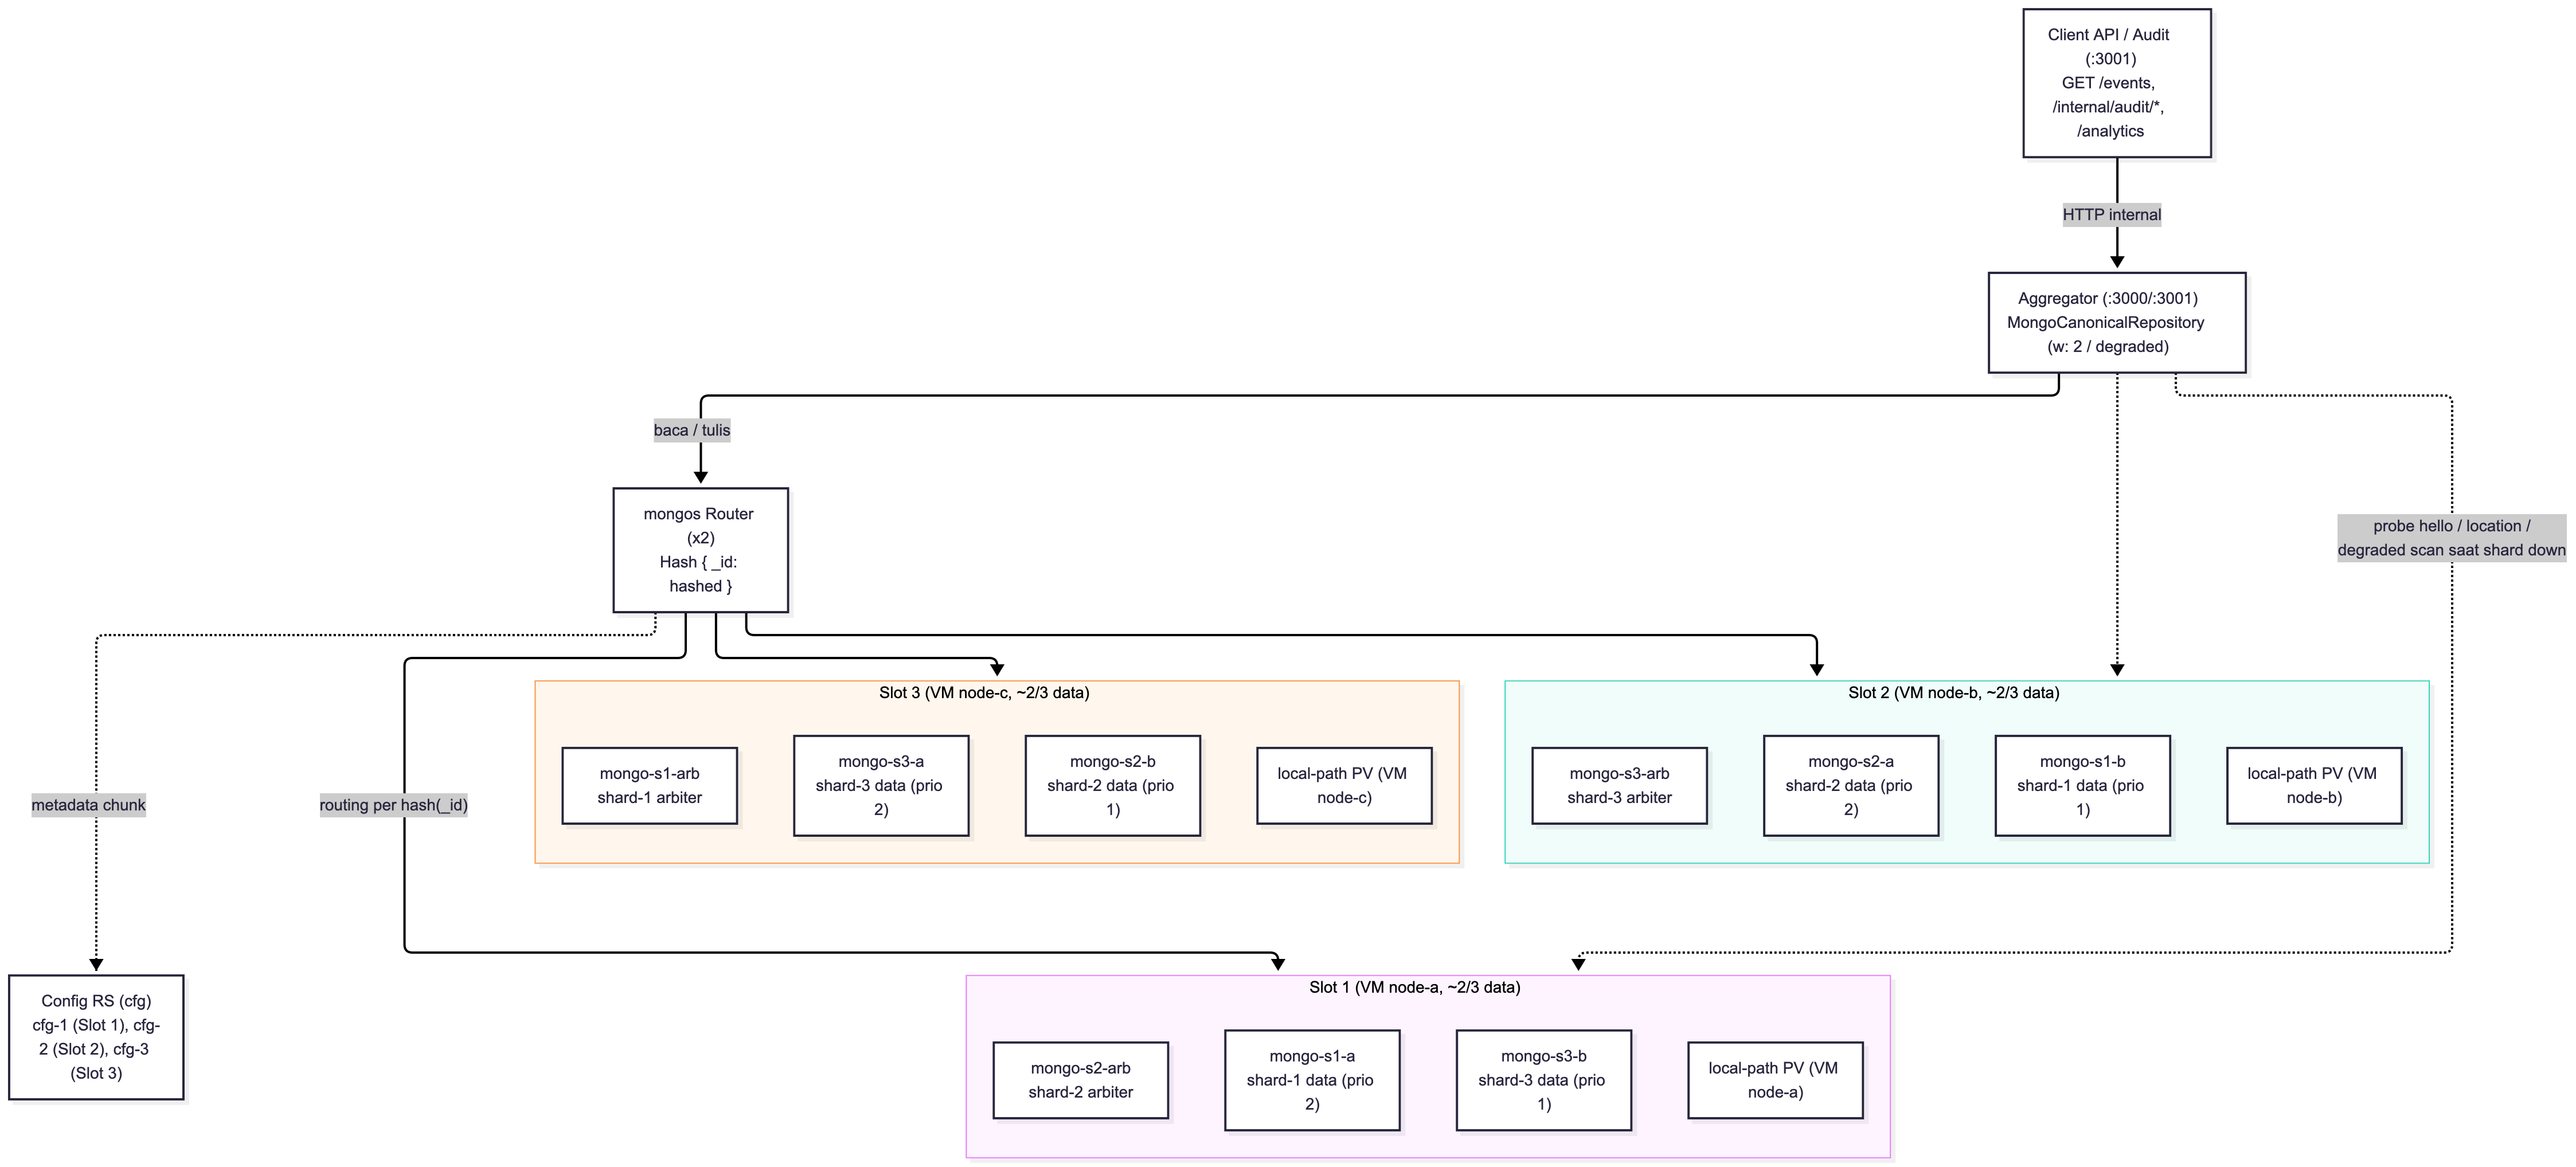
\includegraphics[width=0.95\linewidth]{p1-arsitektur-penyimpanan.png}%
  }{%
  \resizebox{\linewidth}{!}{%
  \begin{tikzpicture}[
    every node/.style={font=\sffamily\footnotesize},
    box/.style={draw=black!65, rounded corners=3pt, fill=white, align=center, inner sep=5pt, minimum width=3.1cm, minimum height=0.9cm},
    member/.style={draw=blue!55!black, rounded corners=2pt, fill=blue!6, align=center, inner sep=4pt, minimum width=3.2cm, minimum height=0.72cm},
    arb/.style={draw=black!50, rounded corners=2pt, fill=black!4, align=center, inner sep=4pt, minimum width=3.2cm, minimum height=0.65cm},
    group/.style={draw=black!40, dashed, rounded corners=4pt, fill=black!2, inner sep=8pt},
    arr/.style={-{Stealth[length=2.2mm]}, thick, draw=black!75},
    lbl/.style={font=\sffamily\scriptsize, fill=white, inner sep=1.5pt, align=center}
  ]
    % Lapisan atas: Client, Aggregator, mongos, Config RS
    \node[box] (api) at (0, 7.0) {\textbf{Client API / Audit (:3001)}\\{\scriptsize GET /events, /internal/audit/*, /analytics}};
    \node[box] (agg) at (6.0, 7.0) {\textbf{Aggregator (:3000/:3001)}\\{\scriptsize MongoCanonicalRepository (w: 2 / degraded)}};
    \node[box] (mongos) at (12.2, 7.0) {\textbf{mongos Router ($\times 2$)}\\{\scriptsize Hash \{ \_id: "hashed" \}}};
    \node[member] (cfg) at (18.4, 7.0) {\textbf{Config RS (\texttt{cfg})}\\{\scriptsize cfg-1 (Slot 1), cfg-2 (Slot 2), cfg-3 (Slot 3)}};

    % Lapisan bawah: 3 Node Slots (node-a, node-b, node-c)
    % Slot 1
    \node[member] (s1a) at (1.5, 3.0) {\textbf{mongo-s1-a}\\{\scriptsize shard-1 data (prio 2)}};
    \node[member] (s3b) at (1.5, 2.0) {\textbf{mongo-s3-b}\\{\scriptsize shard-3 data (prio 1)}};
    \node[arb]    (s2r) at (1.5, 1.0) {\textbf{mongo-s2-arb}\\{\scriptsize shard-2 arbiter}};
    \node[box, minimum height=0.55cm] (pv1) at (1.5, 0.0) {\scriptsize local-path PV (VM node-a)};

    % Slot 2
    \node[member] (s2a) at (9.2, 3.0) {\textbf{mongo-s2-a}\\{\scriptsize shard-2 data (prio 2)}};
    \node[member] (s1b) at (9.2, 2.0) {\textbf{mongo-s1-b}\\{\scriptsize shard-1 data (prio 1)}};
    \node[arb]    (s3r) at (9.2, 1.0) {\textbf{mongo-s3-arb}\\{\scriptsize shard-3 arbiter}};
    \node[box, minimum height=0.55cm] (pv2) at (9.2, 0.0) {\scriptsize local-path PV (VM node-b)};

    % Slot 3
    \node[member] (s3a) at (16.9, 3.0) {\textbf{mongo-s3-a}\\{\scriptsize shard-3 data (prio 2)}};
    \node[member] (s2b) at (16.9, 2.0) {\textbf{mongo-s2-b}\\{\scriptsize shard-2 data (prio 1)}};
    \node[arb]    (s1r) at (16.9, 1.0) {\textbf{mongo-s1-arb}\\{\scriptsize shard-1 arbiter}};
    \node[box, minimum height=0.55cm] (pv3) at (16.9, 0.0) {\scriptsize local-path PV (VM node-c)};

    % Kotak Slot
    \begin{scope}[on background layer]
      \node[group, fit=(s1a)(s3b)(s2r)(pv1), label={[font=\sffamily\scriptsize\bfseries]above:Slot 1 (VM node-a $\cdot$ ~2/3 data)}] (slot1) {};
      \node[group, fit=(s2a)(s1b)(s3r)(pv2), label={[font=\sffamily\scriptsize\bfseries]above:Slot 2 (VM node-b $\cdot$ ~2/3 data)}] (slot2) {};
      \node[group, fit=(s3a)(s2b)(s1r)(pv3), label={[font=\sffamily\scriptsize\bfseries]above:Slot 3 (VM node-c $\cdot$ ~2/3 data)}] (slot3) {};
    \end{scope}

    % Panah utama
    \draw[arr] (api) -- node[lbl, above] {HTTP internal} (agg);
    \draw[arr] (agg) -- node[lbl, above] {baca/tulis} (mongos);
    \draw[arr, dashed] (mongos) -- node[lbl, above] {metadata chunk} (cfg);

    \draw[arr] (mongos.south) -- ++(0,-0.65) -| node[lbl, near start, above] {routing per hash(\_id)} ([yshift=13pt]slot1.north);
    \draw[arr] (mongos.south) -- ++(0,-0.65) -| ([yshift=13pt]slot2.north);
    \draw[arr] (mongos.south) -- ++(0,-0.65) -| ([yshift=13pt]slot3.north);

    % Jalur probe langsung (degraded scan & /audit/location)
    \draw[arr, dashed] (agg.south) -- ++(0,-1.15) -| node[lbl, pos=0.25, above] {probe hello / location / scan saat shard down} ([xshift=-2.3cm, yshift=13pt]slot1.north);
    \draw[arr, dashed] (agg.south) -- ++(0,-1.15) -| ([xshift=-2.3cm, yshift=13pt]slot2.north);
  \end{tikzpicture}%
  }%
  }
  \caption{Diagram Rancangan Solusi Penyimpanan Terdistribusi Problem 1}
  \label{fig:p1-arch}
\end{figure}

Rancangan ini bertumpu pada empat mekanisme utama berikut.

\paragraph*{1. Topologi Tiga \textit{Shard} Terotasi di Atas Tiga Node VM}
Konfigurasi penyimpanan dihasilkan secara deklaratif dari \path{k8s/store/layout.json} melalui \path{k8s/store/generate.mjs} dan diinisialisasi secara \textit{idempotent} oleh \path{k8s/store/init.js}:

\begin{itemize}
  \item \textbf{Rotasi anggota tiap slot:} setiap \textit{shard} (\texttt{shard-1}, \texttt{shard-2}, dan \texttt{shard-3}) terdiri atas dua anggota penyimpan data dan satu \textit{arbiter}. Anggota data terdiri atas \textit{primary} berprioritas 2 dan \textit{secondary} berprioritas 1, sedangkan \textit{arbiter} berprioritas 0. Ketiganya selalu ditempatkan pada tiga \textit{node} berbeda menggunakan label \path{bnpb.io/store-slot=1..3}. Tiap \textit{node} hanya menyimpan sekitar dua pertiga dataset sehingga kehilangan satu \textit{node} tetap menyisakan minimal satu salinan hidup per \textit{shard}.
  \item \textbf{\textit{Router} dan pengatur metadata:} sistem menjalankan dua replika \textit{stateless} \texttt{mongos} pada \textit{node} terpisah melalui \textit{topology spread}. Metadata pembagian \textit{chunk} dikelola oleh satu \textit{replica set} \texttt{cfg} dengan tiga \textit{config server} pada masing-masing slot.
  \item \textbf{Isolasi penyimpanan:} komunikasi antarkomponen di klaster basis data dikunci menggunakan \textit{keyfile} internal. Akses memakai akun berhak minimal (\texttt{aggregator} dan \texttt{probe}), lalu dikunci oleh \texttt{NetworkPolicy} pada \path{k8s/store/policy.yaml} agar hanya Aggregator yang dapat mengakses basis data.
\end{itemize}

\paragraph*{2. \textit{Hashed Sharding} pada Identitas Deterministik \texttt{hazard\_id}}
Pada \path{k8s/store/init.js:65-68}, koleksi \path{bnpb_canonical_store.hazards} dipartisi dengan kunci \path{{ _id: 'hashed' }} memakai enam \textit{initial chunks}. Nilai \texttt{\_id} disamakan dengan \texttt{hazard\_id} deterministik hasil fungsi \texttt{hazardIdFor(source, source\_ref\_id)} di \path{aggregator/src/storage/identity.ts}.

Penempatan \textit{shard} dihitung dari \textit{hash} SHA-256 pasangan sumber dan referensinya, bukan dari koordinat, provinsi, atau waktu kejadian. Karena itu, lonjakan gempa pada satu wilayah tetap tersebar merata ke ketiga \textit{shard}.

\paragraph*{3. Jalur Tulis (\texttt{w: 2}) dan Baca Parsial Terbatas Waktu}
Seluruh operasi baca dan tulis Aggregator dikemas dalam kelas \texttt{MongoCanonicalRepository} di \path{aggregator/src/storage/mongoRepository.ts}.

\begin{itemize}
  \item \textbf{Jalur tulis tahan gangguan (\texttt{ingest}, baris 83--113):} setiap peristiwa disimpan memakai operasi kondisional \texttt{updateOne} beropsi \texttt{upsert: true} dengan \textit{write concern} baku \texttt{w: 2} dan batas waktu \texttt{1500 ms}. Saat kedua anggota data sehat, penulisan baru diakui setelah mendarat di dua replika. Jika satu anggota mati, penulisan ke \textit{primary} menghasilkan \texttt{MongoWriteConcernError} setelah 1,5 detik lalu diakui sebagai \texttt{degraded: true} agar pencatatan tetap berjalan. Mode \textit{fail-closed} dapat diaktifkan lewat \path{STORE_STRICT_WRITES=1}. Operasi ini sekaligus menjaga \texttt{event\_version} dan \texttt{fence\_epoch} secara atomik.
  \item \textbf{Kueri global terurut (\texttt{queryGlobal}, baris 161--212):} kueri daftar terbaru memakai \texttt{readPreference: 'primaryPreferred'} dan pengurutan stabil lewat \textit{keyset cursor} (\path{cursor.ts}). Perintah ini menyertakan \texttt{allowPartialResults: true} serta memotong \texttt{maxTimeMS} menjadi $600\text{ ms}$ apabila pemantau latar belakang mendeteksi ada \textit{shard} mati. Hasil \texttt{partialResultsReturned} maupun unit mati diteruskan menjadi properti \texttt{partial: true} dan \texttt{unavailable\_units} di \path{GET /events} (\path{client-api/src/routes/events.ts:54-57}).
  \item \textbf{Pemindaian normal dan terdegradasi (\texttt{scan}, baris 219--300):} saat seluruh unit sehat, Audit API dan analitik membaca bertahap lewat \texttt{mongos} menggunakan kunci \texttt{\_id} agar dokumen yatim (\textit{orphan}) saat migrasi \textit{chunk} otomatis tersaring. Apabila ada unit mati, memanggil \texttt{mongos} untuk pemindaian penuh akan tertahan menunggu batas waktu. Oleh karena itu, \texttt{scan} langsung menghubungi anggota hidup tiap unit memakai akun \texttt{probe}, melakukan deduplikasi \texttt{\_id} di memori, lalu mengembalikan batas bawah dalam batas waktu \texttt{scanDeadlineMs} ($8.000\text{ ms}$).
\end{itemize}

\paragraph*{4. Pemulihan Node Pengganti, Audit API, dan Dasbor Analitik}
Skrip \path{scripts/m2/p1-replace-node.sh} mengotomatiskan penggantian \textit{node} dengan disk kosong. Skrip memindahkan label \path{bnpb.io/store-slot} ke \textit{node} baru, menghapus \textit{pod} serta PVC lama, lalu menghidupkan kembali \textit{StatefulSet} terkait agar MongoDB menjalankan \textit{initial sync}. Setelah itu, \path{scripts/m2/store-topology.sh} memperbarui peta penempatan \textit{node}.

Pada sisi observabilitas data, \texttt{createStorageRouter} (\path{aggregator/src/storage/routes.ts}) menyediakan seluruh \textit{endpoint} Audit API Lampiran A serta \path{/internal/analytics/summary}. Halaman HTML mandiri \path{/analytics} (\path{analyticsPage.ts}) menyajikan grafik waktu per jenis bahaya, tabel per tingkat keparahan dan \path{area\_name}, spanduk ``\texttt{DATA BELUM LENGKAP}'', serta tombol rekonsiliasi ke Audit API.

\subsubsection{Alasan Keputusan}

\textbf{Tabel~\ref{tab:p1-decisions}} merangkum keputusan desain utama pada Problem 1, alasan beserta konsekuensinya, dan alternatif yang ditolak.

\begin{small}
\begin{longtable}{@{} >{\raggedright\arraybackslash}p{3.4cm} >{\raggedright\arraybackslash}p{7.4cm} >{\raggedright\arraybackslash}p{4.0cm} @{}}
  \caption{Desain, Alasan, dan Alternatif yang Ditolak pada Problem 1}
  \label{tab:p1-decisions} \\
  \toprule
  \textbf{Keputusan} & \textbf{Alasan} & \textbf{Alternatif (Ditolak)} \\
  \midrule
  \endfirsthead
  \caption[]{Desain, Alasan, dan Alternatif yang Ditolak pada Problem 1 (Lanjutan)} \\
  \toprule
  \textbf{Keputusan} & \textbf{Alasan} & \textbf{Alternatif (Ditolak)} \\
  \midrule
  \endhead
  \midrule
  \multicolumn{3}{r}{\textit{Bersambung ke halaman berikutnya...}} \\
  \endfoot
  \bottomrule
  \endlastfoot
  MongoDB \textit{Sharded Cluster} 3 \textit{shard} terotasi (2 data dan 1 \textit{arbiter}) pada 3 VM & Dengan dua salinan ($R \ge 2$) dan tiga \textit{shard} berotasi, tiap \textit{node} hanya memegang sekitar dua pertiga dataset. Saat satu \textit{node} mati, ketiga \textit{shard} tetap menyisakan minimal satu anggota data aktif. Konsekuensinya, \textit{shard} terdampak hanya memiliki satu salinan hidup sampai \textit{node} pengganti selesai dibangun ulang. & \textbf{CockroachDB:} dengan $RF=3$ setiap \textit{node} memegang semua data, sedangkan dengan $RF=2$ hilangnya satu \textit{node} langsung memutus kuorum. \textbf{3 \textit{data member} per \textit{shard}:} menaruh 100\% dataset di tiap \textit{node}. \\
  \midrule
  Memakai \textit{hashed shard key} \texttt{\{\_id: "hashed"\}} berbasis \texttt{hazard\_id} deterministik & Pembagian berdasarkan \textit{hash} pasangan \texttt{(source, source\_ref\_id)} menyebar beban tulis secara seimbang tanpa dipengaruhi lokasi gempa ataupun urutan waktu. Cara ini juga menjaga keunikan global \texttt{\_id}. Konsekuensinya, kueri saringan wilayah atau rentang waktu tetap menjalankan \textit{scatter-gather} ke ketiga \textit{shard}. & \textbf{\textit{Range shard key} berbasis wilayah:} penumpukan kejadian di satu daerah memusatkan beban tulis pada satu \textit{shard}. \textbf{\textit{Shard key} waktu menaik:} seluruh tulis baru masuk ke \textit{shard} paling ujung. \\
  \midrule
  \textit{Write concern} \texttt{w: 2} (\texttt{1500 ms}) dengan pengakuan \texttt{degraded} & Pada kondisi sehat, \texttt{w: 2} menjamin penulisan tersimpan di kedua anggota data sebelum diakui. Saat satu anggota mati, \texttt{w: majority} tidak dapat terpenuhi sehingga pengakuan \textit{primary} sebagai \texttt{degraded} mempertahankan ketersediaan jalur tulis. & \textbf{\texttt{w: 1} bawaan:} berisiko menganggap aman tulisan satu salinan saat klaster sehat. \textbf{\textit{Fail-closed} (\path{STORE_STRICT_WRITES=1}):} memblokir penulisan ke \textit{shard} terdampak selama pemulihan. \\
  \midrule
  \textit{Router} \texttt{mongos} untuk kondisi normal dan pemindaian paralel saat unit mati & Membaca lewat \texttt{mongos} menyaring dokumen \textit{orphan} saat migrasi \textit{chunk} serta menjaga keutuhan \textit{keyset pagination}. Saat suatu \textit{shard} mati, pemindaian penuh dialihkan langsung ke anggota hidup dengan deduplikasi \texttt{\_id} agar jawaban parsial kembali cepat tanpa menunggu batas waktu. & \textbf{\textit{Sharding} manual di aplikasi:} memaksa aplikasi membangun ulang logika penyeimbang dan penyaringan \textit{orphan}. \textbf{Driver \textit{cursor} standar:} menyembunyikan penanda \texttt{partial\allowbreak Results\allowbreak Returned}. \\
  \midrule
  Dua anggota data plus satu \textit{arbiter} dengan \textit{initial sync} & Kehadiran \textit{arbiter} memungkinkan pemilihan \textit{primary} otomatis saat satu anggota mati tanpa perlu menyimpan salinan ketiga yang melanggar batas sebaran \textit{node}. Konsekuensinya, pada \textit{shard} yang kehilangan satu anggota, \textit{majority commit point} tertahan hingga sinkronisasi ulang selesai. & Menjalankan \textit{replica set} tanpa \textit{arbiter} (kuorum pemilihan gagal saat satu dari dua anggota mati) atau memakai penyimpanan jaringan bersama (tidak menguji disk lokal). \\
\end{longtable}
\end{small}

\subsubsection{Batasan yang Disadari}

\textbf{Tabel~\ref{tab:p1-limits}} merangkum batasan teknis yang disadari pada implementasi Problem 1.

\begin{table}[H]
  \centering
  \caption{Batasan Implementasi yang Disadari pada Problem 1}
  \label{tab:p1-limits}
  \small
  \begin{tabularx}{\linewidth}{@{} >{\raggedright\arraybackslash}p{3.4cm} >{\raggedright\arraybackslash}X >{\raggedright\arraybackslash}p{4.3cm} @{}}
    \toprule
    \textbf{Batasan} & \textbf{Penjelasan dan Alasan} & \textbf{Referensi Kode} \\
    \midrule
    \textbf{Masa \textit{degraded write} bersalinan tunggal} & Saat satu \textit{node} mati dan belum diganti, tulisan baru pada \textit{shard} terdampak hanya tersimpan di satu \textit{primary} (\texttt{degraded: true}). Jika \textit{node} kedua ikut mati sebelum sinkronisasi tuntas, tulisan selama jeda tersebut berisiko hilang. & \path{docs/m2-details/consistency.md:8}, \path{aggregator/src/storage/mongoRepository.ts:104-109} \\
    \midrule
    \textbf{Pembacaan berpotensi \textit{stale read} sesaat} & Kueri memakai \texttt{primaryPreferred} dan \textit{read concern} \texttt{local}. Pembacaan dari \textit{secondary} atau sesaat setelah pergantian \textit{primary} dapat tertinggal tipis dari oplog terbaru, meski tulisan berstatus \texttt{w: 2} tetap aman. & \path{docs/m2-details/consistency.md:17-18} \\
    \midrule
    \textbf{Analitik dan \texttt{checksum} bukan \textit{snapshot} terisolasi} & Pemindaian menyeluruh memakai urutan kunci \texttt{\_id} dalam anggaran waktu $8.000\text{ ms}$ dengan stempel waktu \texttt{as\_of}. Bila penulisan aktif berlangsung bersamaan, perbandingan \texttt{checksum} dilakukan saat aliran tulis dihentikan sementara. & \path{docs/m2-details/consistency.md:11-12}, \path{aggregator/src/storage/mongoRepository.ts:219-317} \\
    \midrule
    \textbf{Otomatisasi penggantian hanya untuk tiga slot tetap} & Skrip \path{p1-replace-node.sh} dirancang untuk menggantikan salah satu dari tiga slot yang ada. Penambahan \textit{node} keempat sebagai \textit{shard} baru berkapasitas ekstra belum diotomatiskan oleh skrip. & \path{docs/m2-details/decisions/ADR-0001-storage.md:42}, \path{scripts/m2/p1-replace-node.sh:1-12} \\
    \bottomrule
  \end{tabularx}
\end{table}

\subsubsection{Bukti Penyelesaian per Kriteria}

Bukti berikut berasal dari eksekusi skrip pada klaster tiga VM (\texttt{node-a}, \texttt{node-c}, \texttt{node-d}). Keluaran teks lengkap tiap eksekusi tersimpan di repositori pada \path{docs/m2-details/proofs/}. Dataset katalog gempa resmi dari asisten belum tersedia, sehingga Kriteria 1 hingga 6 memakai katalog simulasi 50.000 kejadian yang dimuat melalui jalur \textit{ingest} yang sama.


\paragraph*{Kriteria 1: sebaran data per \textit{node}.}
\path{p1-report.sh} melaporkan 155.322 rekaman logis dengan salinan per \textit{node} sebanyak 103.494 (\texttt{node-a}), 103.477 (\texttt{node-d}), dan 103.587 (\texttt{node-c}). Pangsa terbesar satu \textit{node} adalah 0,667 dari dataset, sehingga tidak ada \textit{node} yang menyimpan seluruh data. Setiap \textit{shard} memiliki \textit{primary} dan \textit{secondary} pada \textit{node} berbeda.
\gambarbukti{bk-1-1.png}{Sebaran data per \textit{node} dan lokasi salinan (\texttt{p1-report.sh})}{bk-1-1}

\paragraph*{Kriteria 2: ketidakmerataan beban.}
\path{p1-hotspot.sh} menulis 20.000 kejadian dari satu wilayah (Sumatera Barat). Tiap \textit{primary} menerima 8.284 (\texttt{shard-1}), 6.983 (\texttt{shard-2}), dan 6.941 (\texttt{shard-3}) penulisan. Rasio maksimum terhadap minimum adalah 1,19 (batas lulus $< 2$), sehingga lonjakan satu wilayah tidak memusatkan beban pada satu \textit{node}.
\gambarbukti{bk-1-2.png}{Beban tulis per \textit{primary} saat lonjakan satu wilayah (\texttt{p1-hotspot.sh})}{bk-1-2}

\paragraph*{Kriteria 3: baca lintas penyimpanan dan \textit{pagination}.}
\path{p1-query.sh} menelusuri Audit API sepanjang 354 halaman (176.915 rekaman) tanpa duplikat dan tanpa pelanggaran urutan \path{(ingested_at, hazard_id)}. Permintaan 50 kejadian terbaru lintas jenis bahaya juga berurutan benar dan lengkap (\texttt{partial = false}).
\gambarbukti{bk-1-3.png}{Urutan global dan \textit{pagination} lintas penyimpanan (\texttt{p1-query.sh})}{bk-1-3}

\paragraph*{Kriteria 4: node mati dan disk terhapus.}
Seluruh anggota penyimpanan pada satu slot dihentikan dan volumenya dihapus. Selama pemulihan terdapat 52 jawaban lengkap dan 2 jawaban \texttt{partial: true} yang ditandai eksplisit, 18 pembacaan \textit{client API} berhasil, dan 0 jawaban 5xx atau menggantung. Jumlah rekaman 176.957 menjadi 177.053 dengan 0 rekaman hilang. Pada uji kedua, satu \textit{shard} utuh dibuat tidak terjangkau: seluruh jawaban ditandai \texttt{partial: true} dengan \texttt{unavailable\_units} berisi \texttt{shard-1}, tanpa 5xx, dan data kembali utuh setelah dipulihkan. Perbandingan terhadap \textit{checksum} resmi asisten menunggu bahan pengujian dari asisten; pembandingan ini memakai rekaman sebelum dan sesudah kehilangan.
\gambarbukti{bk-1-4.png}{Kehilangan slot dan penggantian volume kosong (\texttt{p1-node-loss.sh})}{bk-1-4}
\gambarbukti{bk-1-4p.png}{Satu \textit{shard} tidak terjangkau: jawaban \textit{partial} eksplisit (\texttt{p1-unit-loss.sh})}{bk-1-4p}

\paragraph*{Kriteria 5: node pengganti berdisk kosong tanpa menghentikan baca dan tulis.}
Saat slot yang sama diganti dengan volume kosong, satu tulisan laporan lapangan dikirim tiap 0,5 detik: 496 dari 496 dijawab 202 (p95 0,07 detik), seluruhnya tersimpan tanpa duplikat. Pembacaan pada periode itu berjumlah 45 jawaban lengkap dan 3 jawaban \textit{partial} eksplisit, dengan 0 rekaman hilang.
\gambarbukti{bk-1-5.png}{Penulisan dan pembacaan selama sinkronisasi awal (\texttt{p1-write-probe.sh})}{bk-1-5}

\paragraph*{Kriteria 6: ketahanan terhadap kehilangan node berikutnya.}
Setelah slot pertama pulih penuh, slot kedua diperlakukan sama: 51 jawaban lengkap, 17 pembacaan \textit{client API} berhasil, 0 jawaban buruk, dan rekaman 177.780 menjadi 177.853 dengan 0 hilang.
\gambarbukti{bk-1-6.png}{Kehilangan \textit{node} berikutnya setelah pemulihan (\texttt{p1-node-loss.sh 2})}{bk-1-6}

\paragraph*{Kriteria 7: dasbor analitik.}
Dasbor menampilkan grafik per jenis bahaya, jumlah per \textit{severity}, dan jumlah per \texttt{area\_name} dengan spanduk hijau ``Data lengkap''. Tombol ``Cocokkan dengan Audit API'' menunjukkan angka yang sama (64.814 melawan 64.814, ``COCOK''). Saat satu \textit{shard} tidak terjangkau, spanduk berubah menjadi ``DATA BELUM LENGKAP: unit tidak terjangkau (shard-1)'' dan angkanya disebut batas bawah. Setelah pemulihan spanduk kembali hijau.
\gambarbukti[0.30]{bk-1-7a.png}{Dasbor analitik lengkap (rentang 24 jam)}{bk-1-7a}
\gambarbukti[0.30]{bk-1-7b.png}{Kecocokan angka dasbor dengan Audit API}{bk-1-7b}
\gambarbukti[0.30]{bk-1-7c.png}{Spanduk data belum lengkap saat satu \textit{shard} mati}{bk-1-7c}
\gambarbukti[0.30]{bk-1-7d.png}{Dasbor kembali lengkap setelah pemulihan}{bk-1-7d}

\subsubsection{Jawaban atas Butir ``Di laporan''}

\paragraph*{Persoalan Inti Penyimpanan Terdistribusi dan Pilihan Kunci Partisi}
Problem 1 mempertemukan empat persoalan klasik penyimpanan terdistribusi. Pertama adalah \textit{data partitioning} beserta anomali \textit{partition skew} atau \textit{write-read hotspot} akibat sifat data gempa yang mengelompok secara geografis. Kedua adalah \textit{replication} dan \textit{fault tolerance} terhadap hilangnya mesin beserta disk lokal, yang menuntut \textit{graceful degradation}. Ketiga adalah \textit{distributed scatter-gather query} dengan \textit{keyset pagination} dan agregasi bebas duplikasi. Keempat adalah \textit{online rebalancing} dan \textit{replica initial sync} saat \textit{node} pengganti masuk tanpa memutus layanan.

Untuk mencegah \textit{write hotspot}, sistem memilih \textit{\textbf{hashed shard key}} pada \path{{ _id: 'hashed' }} (\path{k8s/store/init.js:67}). Nilai \texttt{\_id} diturunkan dari \textit{hash} SHA-256 pasangan \texttt{(source, source\_ref\_id)}. Karena hasil \textit{hash} seragam, lonjakan ribuan gempa di satu koordinat atau provinsi tetap terbagi rata ke \texttt{shard-1}, \texttt{shard-2}, dan \texttt{shard-3}.

Dua pendekatan lain ditolak karena gagal menangani Kriteria 2. Pendekatan \textit{range shard key} berdasarkan \texttt{area\_name} atau koordinat memusatkan seluruh lonjakan gempa wilayah tertentu ke satu \textit{chunk} dan satu \textit{shard} saja. Pendekatan kunci waktu menaik seperti \texttt{occurred\_at} atau ID berurutan juga memicu \textit{single-shard write bottleneck} karena setiap catatan baru selalu mendarat di \textit{chunk} paling ujung.

\paragraph*{Dinamika Lokasi Data Saat Node Pergi dan Datang}
Router \texttt{mongos} memetakan rentang \textit{hash} 64-bit ke enam \textit{initial chunks} di antara ketiga \textit{shard} berdasarkan metadata \textit{Config Server} (\texttt{cfg}). Sesuai \path{k8s/store/layout.json}, tiap \textit{shard} menempatkan dua anggota penyimpan data pada dua slot VM berbeda dan satu \textit{arbiter} pada slot sisanya.

Ketika satu \textit{node} mati permanen, satu anggota data pada dua \textit{shard} serta satu \textit{arbiter} ikut hilang. Dua \textit{node} yang masih hidup tetap menyimpan minimal satu salinan aktif untuk setiap \textit{shard}. Pembacaan tetap dilayani oleh anggota tersisa, sementara penulisan ke \textit{shard} terdampak ditandai sebagai \texttt{degraded: true} pada \textit{primary} hidup. Unit yang tidak terjangkau dicatat dalam daftar \texttt{unavailable\_units}.

Ketika \textit{node} baru dengan disk kosong hadir, \path{scripts/m2/p1-replace-node.sh} memindahkan label slot ke \textit{node} pengganti dan membuat volume baru bagi \textit{pod} \textit{StatefulSet} slot tersebut. MongoDB lalu menjalankan \textit{initial sync} otomatis untuk menyalin dokumen dan oplog tanpa mematikan layanan baca atau tulis. Terakhir, \path{store-topology.sh} menyegarkan peta penempatan untuk \path{/internal/audit/location}.

\paragraph*{Jaminan Konsistensi per \textit{Endpoint} dan Perhitungan Dasbor Analitik}
Pada kondisi normal maupun terdegradasi, tiap \textit{endpoint} menerapkan jaminan konsistensi terukur sebagai berikut:

\begin{itemize}
  \item \textbf{Penulisan kanonik (\texttt{repo.ingest}):} kondisi normal menjamin durabilitas dua salinan sebelum diakui (\texttt{w: 2}) serta keunikan \textit{idempotent} atas \texttt{hazard\_id}. Saat satu \textit{node} mati, tulis pada \textit{shard} terdampak diakui sebagai \texttt{degraded: true} di \textit{primary} hidup, kecuali jika \path{STORE_STRICT_WRITES=1} diaktifkan.
  \item \textbf{Daftar kejadian publik (\path{GET /events}):} kondisi normal menjaga urutan global \path{(occurred_at desc, hazard_id)} dengan semantik \textit{eventual read} akibat \texttt{primaryPreferred} dan \textit{read concern} \texttt{local}. Jika ada unit mati atau melampaui batas $600\text{ ms}$, \textit{endpoint} tetap menjawab dengan \texttt{partial: true} dan daftar \texttt{unavailable\_units}.
  \item \textbf{Audit daftar dan penelusuran (\path{GET /internal/audit/events} dan \path{/checksum}):} mengembalikan urutan \path{(ingested_at, hazard_id)} atau nilai \textit{hash} SHA-256 \texttt{source\_ref\_id} terurut secara non-\textit{snapshot} dengan stempel \texttt{as\_of}. Bila sebagian unit mati, kedua \textit{endpoint} menyertakan \texttt{partial: true} sehingga pembanding tahu hasilnya tidak utuh.
  \item \textbf{Audit lokasi (\path{GET /internal/audit/location}):} menghubungi tiap anggota data secara langsung untuk memetakan nama \textit{pod} dan \textit{node} Kubernetes. Anggota yang mati dihilangkan dari daftar, dan flag \texttt{partial: true} muncul jika tidak ada satu pun anggota yang dapat dihubungi.
\end{itemize}

Dasbor \path{GET /analytics} menarik ringkasan dari \path{GET /internal/analytics/summary} dan \texttt{aggregate} di \path{aggregator/src/storage/mongoRepository.ts:302-308}. Saat klaster sehat, fungsi \texttt{scan} menyusuri seluruh koleksi melalui \texttt{mongos} dengan kunci \texttt{\_id} sehingga dokumen \textit{orphan} tersaring dan setiap kejadian hanya dihitung satu kali ke dalam \texttt{AnalyticsAccumulator} (\path{analytics.ts:20-61}). Angka turunan \texttt{tsunami\_flagged} dihitung tanpa menggandakan total kejadian.

Ketika pemantau mendeteksi ada unit mati, \texttt{scan} langsung membaca seluruh unit hidup secara paralel memakai akun \texttt{probe} dengan himpunan deduplikasi \texttt{\_id} di memori. Mekanisme ini memastikan salinan replika tidak pernah terhitung ganda sambil menjaga batas waktu $8.000\text{ ms}$. Jika ada bagian yang terputus, \path{analyticsPage.ts:34-36} menampilkan spanduk kuning ``\texttt{DATA BELUM LENGKAP}'' beserta tombol verifikasi silang ke Audit API.
